\documentclass[varwidth=true, border=10pt]{standalone}
\usepackage{tkz-euclide}
\usepackage{tikz}
\usetikzlibrary{patterns}

\begin{document}
\usetkzobj{all}
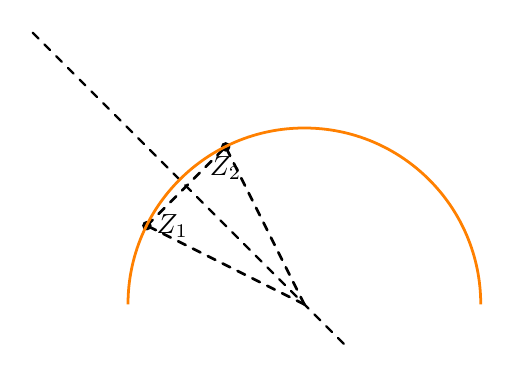
\begin{tikzpicture}
    \tkzSetUpPoint[shape=circle,size=3,color=black,fill=black]
    \tkzSetUpLine[line width=1]
    \tkzInit[xmax=5,ymax=4,xmin=-1,ymin=0]
    \tkzDefPoints{1/1/Z1,2/2/Z2,3/0/A}
    \tkzAxeXY

    \tkzDrawPoints(Z1, Z2)
    \tkzLabelPoint[right](Z1){$Z_1$}
    \tkzLabelPoint[below](Z2){$Z_2$}
    \node (m) at ($(Z1)!0.5!(Z2)$) {};
    \tkzDrawSegments[dashed](Z1,Z2 A,Z1 A,Z2)

    \tkzDefLine[perpendicular=through m](Z1,Z2)\tkzGetPoint{c}
    \tkzDrawLine[add=2 and 1,dashed,thick](m, c)
    \tkzDrawArc[R,line width=1pt,color=orange](A,2.24 cm)(0,180)
\end{tikzpicture}
\end{document}
